%%---------------Homework Template------------------%%
%----------------------------------------------------%
\documentclass[a4paper,9pt]{article}

%---------------code settings------------------------%
\usepackage{listings}
\usepackage{xcolor}
\definecolor{mygreen}{rgb}{0,0.6,0}
\definecolor{mygray}{rgb}{0.5,0.5,0.5}
\definecolor{mymauve}{rgb}{0.58,0,0.82}

\lstset{ %
  backgroundcolor=\color{white},   % choose the background color; you must add \usepackage{color} or \usepackage{xcolor}
  basicstyle=\footnotesize,        % the size of the fonts that are used for the code
  breakatwhitespace=false,         % sets if automatic breaks should only happen at whitespace
  breaklines=true,                 % sets automatic line breaking
  captionpos=bl,                    % sets the caption-position to bottom
  commentstyle=\color{mygreen},    % comment style
  deletekeywords={...},            % if you want to delete keywords from the given language
  escapeinside={\%*}{*)},          % if you want to add LaTeX within your code
  extendedchars=true,              % lets you use non-ASCII characters; for 8-bits encodings only, does not work with UTF-8
  frame=single,                    % adds a frame around the code
  keepspaces=true,                 % keeps spaces in text, useful for keeping indentation of code (possibly needs columns=flexible)
  keywordstyle=\color{blue},       % keyword style
  %language=Python,                 % the language of the code
  morekeywords={*,...},            % if you want to add more keywords to the set
  numbers=left,                    % where to put the line-numbers; possible values are (none, left, right)
  numbersep=5pt,                   % how far the line-numbers are from the code
  numberstyle=\tiny\color{mygray}, % the style that is used for the line-numbers
  rulecolor=\color{black},         % if not set, the frame-color may be changed on line-breaks within not-black text (e.g. comments (green here))
  showspaces=false,                % show spaces everywhere adding particular underscores; it overrides 'showstringspaces'
  showstringspaces=false,          % underline spaces within strings only
  showtabs=false,                  % show tabs within strings adding particular underscores
  stepnumber=1,                    % the step between two line-numbers. If it's 1, each line will be numbered
  stringstyle=\color{orange},     % string literal style
  tabsize=2,                       % sets default tabsize to 2 spaces
  %title=myPython.py                   % show the filename of files included with \lstinputlisting; also try caption instead of title
}

%---------------------other package--------------&
\usepackage[T1]{fontenc}
\usepackage[utf8x]{inputenc}
\usepackage[english]{babel}
\usepackage{float}
\usepackage[colorlinks=true, allcolors=blue]{hyperref}
\usepackage[parfill]{parskip}
\usepackage[a4paper,top=2cm,bottom=3cm,left=1.5cm,right=1.5cm,marginparwidth=2cm]{geometry}
\usepackage{graphicx}
\usepackage{subfigure}
\usepackage{fancyhdr}
\usepackage{titlesec}
\usepackage{amsmath}
\usepackage{amssymb}
\usepackage{indentfirst}
\setlength{\headheight}{41pt}
\setlength{\parindent}{2em}


\begin{document}

%--------------fancyhead------------%
\pagestyle{fancy}
\fancyhead[R]{Classical Electrondynamics}
\fancyhead[L]{
\includegraphics[width=4.5cm]{logo/row.png}}
\fancyfoot[R]{
\includegraphics[width=3cm]{logo/spst.png}}
%---------------title---------------%
\title{\textbf{\Huge{Homework-3}}}

%--------------author---------------%
\author{\textit{Xinzhi Li} \\\quad\\Student ID:~~$\boldsymbol{2022211084}$\\\quad\\ \textit{School of Physics Science and Technology, ShanghaiTech University, Shanghai 201210, China}\\\quad \\ \textit{Email address}:\quad lixzh2022@shanghaitech.edu.cn}


%---------------Logo----------------%
\begin{figure*}[t]
\centering

\includegraphics[width=1\columnwidth]{logo/row.png}
\end{figure*}

%--------------maketitle--------------&
\maketitle\thispagestyle{empty}
%--------------main body--------------&
\newpage
\setcounter{page}{1}

\begin{enumerate}
  \item \textbf{Multipoles}
  \begin{enumerate}
    \item Please calculate the total charge, dipole moment and quadrupole moment for the charge distributions shown in two figure (a) and (b).
    \item Please expand the electrostatic potential in fig.(b) using multipole expansion, clarify the different contributions from total charge, dipole moments. Plot the potential (in terms of multipole expansion) in the $x$-$y$ plane as a function of distance $r$ for $r>a$. Compare this with the exact result calculated using Coulomb's law.
    \begin{figure}[h]
      \begin{minipage}[t]{0.45\linewidth}
        \centering
        \subfigure[]{
        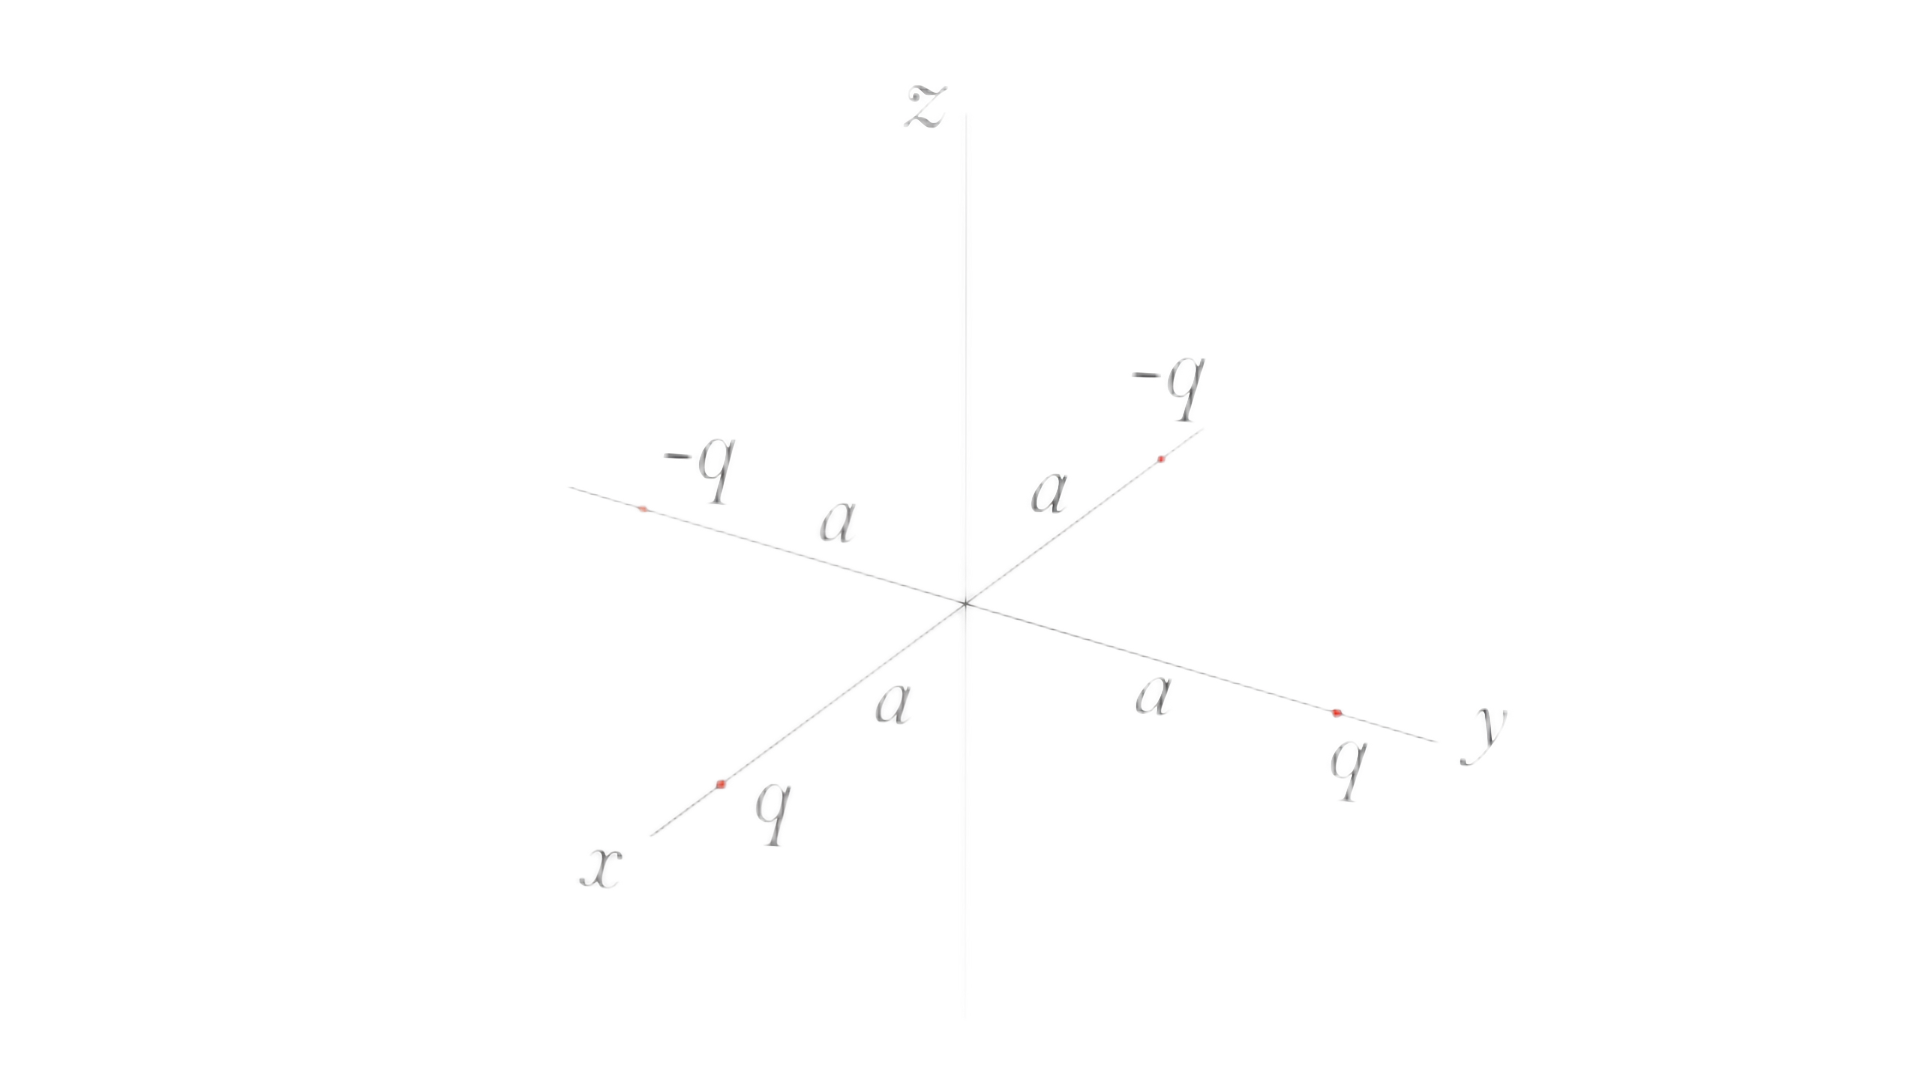
\includegraphics[width=0.9\textwidth]{1.png}
      }
      \end{minipage}
      \hfill
      \begin{minipage}[t]{0.45\linewidth}
        \centering
        \subfigure[]{
        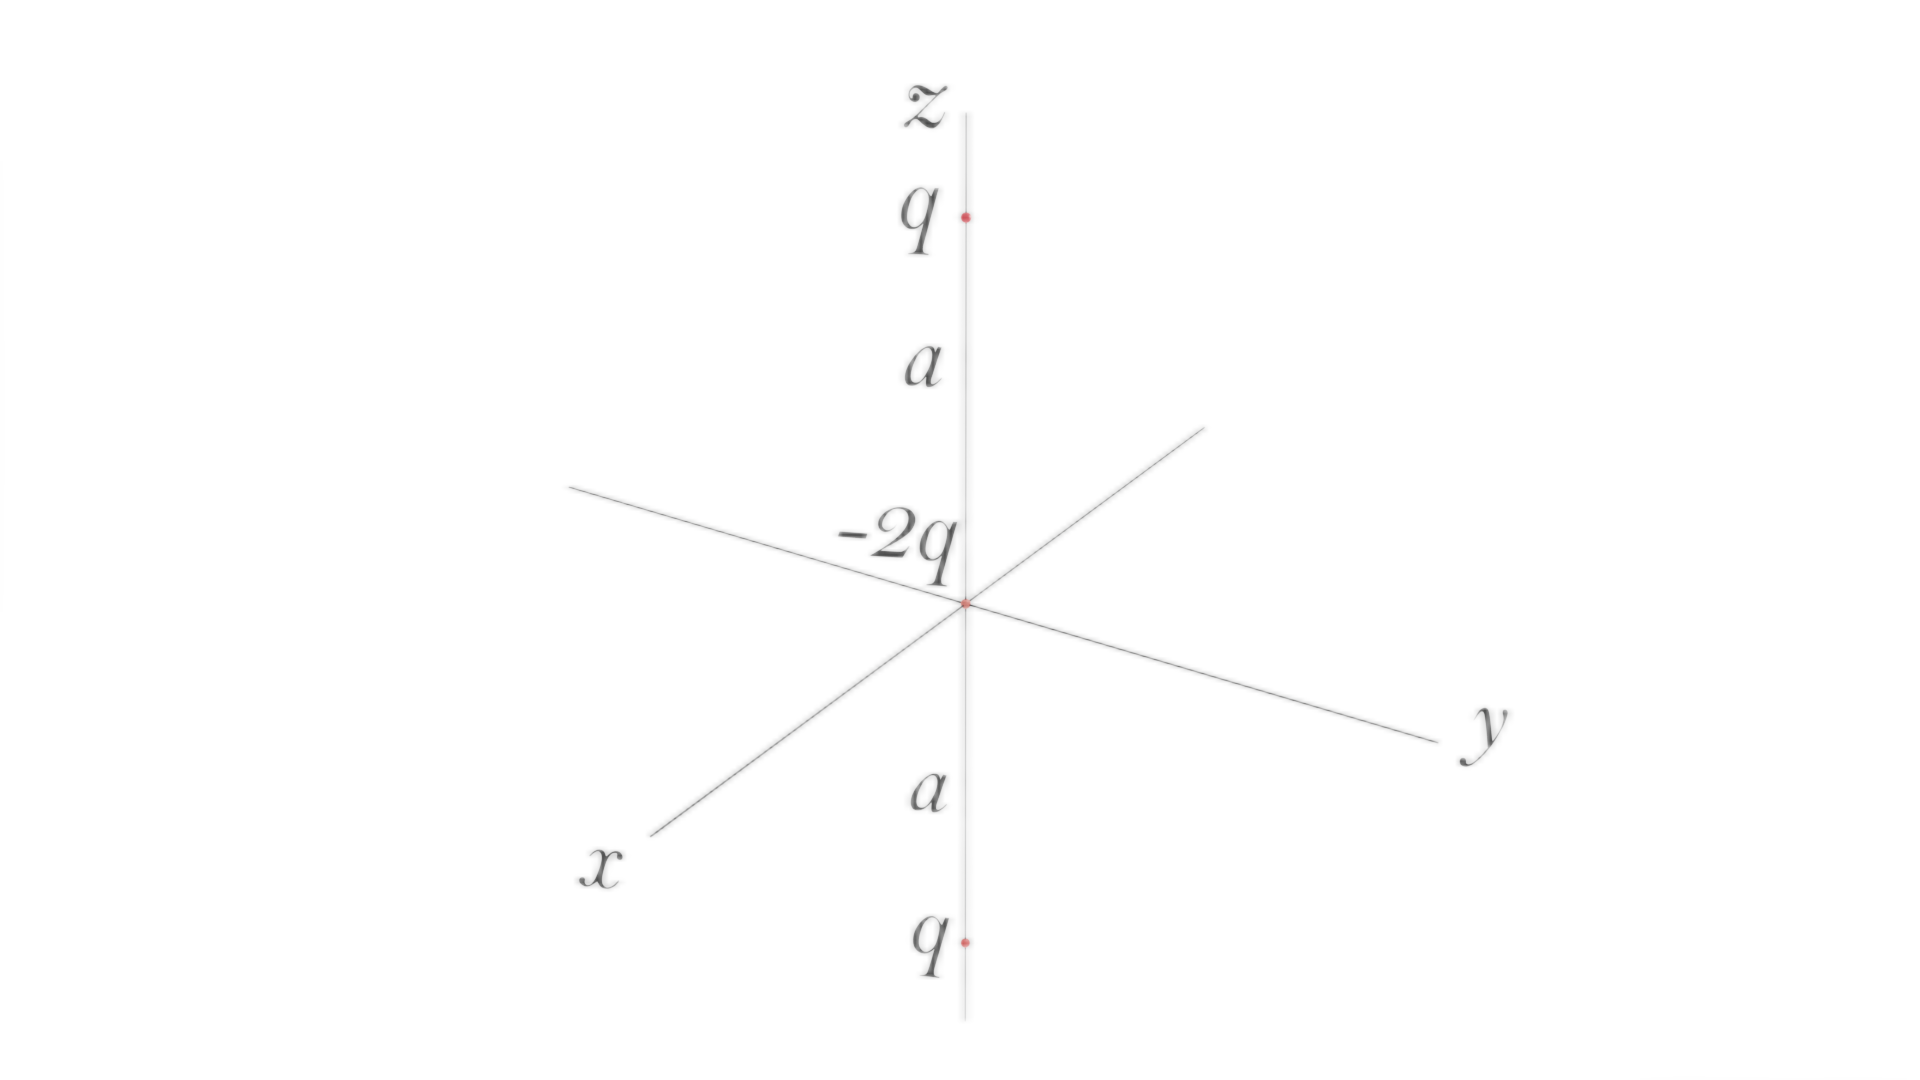
\includegraphics[width=0.9\textwidth]{2.png}
      }
      \end{minipage}
      
    \end{figure}\label{fig1}
  \end{enumerate}
  \rule[0pt]{6cm}{0.05em}
  \begin{enumerate}
    \item  The total charge in (a):
    \begin{eqnarray}
      Q=\int d\boldsymbol{r}'\rho(\boldsymbol{r}')=\int d\boldsymbol{r}' q\left[\delta(y'-a)+\delta(x'-a)-\delta(y'+a)-\delta(x'+a)\right]=0
    \end{eqnarray}
    
    The dipole moment in (a):
    \begin{eqnarray}
      \boldsymbol{p}=\int d\boldsymbol{r}'\rho(\boldsymbol{r}')\boldsymbol{r}'=\int d\boldsymbol{r}'q\left[\delta(y'-a)+\delta(x'-a)-\delta(y'+a)-\delta(x'+a)\right]\boldsymbol{r}'=2qa\hat{\boldsymbol{x}}+2qa\hat{\boldsymbol{y}}
    \end{eqnarray}

    The quadrupole moment in (a):
    \begin{eqnarray}
      \mathcal{Q}_{ij}=\int d\boldsymbol{r}'(3x'_{i}x'_{j}-r'^2\delta_{ij})\rho(\boldsymbol{r}')=0
    \end{eqnarray}

    Similarly, for (b):
    \begin{eqnarray}
      Q&=&0\\
      \boldsymbol{p}&=&0\\
      \mathcal{Q}_{33}=-2\mathcal{Q}_{22}=-2\mathcal{Q}_{11}=4a^2q&,&\quad\mathcal{Q}_{12}=\mathcal{Q}_{21}=\mathcal{Q}_{13}=\mathcal{Q}_{31}=\mathcal{Q}_{32}=\mathcal{Q}_{23}=0
    \end{eqnarray}

    \item The electrostatic potential is 
    \begin{eqnarray}
      \varphi(\boldsymbol{r})&=&\int d\boldsymbol{r}'\dfrac{\rho(\boldsymbol{r}')}{4\pi\epsilon_0|\boldsymbol{r}-\boldsymbol{r}'|}\nonumber\\
      &=&\dfrac{1}{4\pi\epsilon_0}\int d\boldsymbol{r}'\rho(\boldsymbol{r}')(\dfrac{1}{r}+\boldsymbol{r}'\cdot\dfrac{\boldsymbol{r}}{r^3}+\dfrac{1}{2}\sum_{i,j}x'_i x'_j\dfrac{\partial^2}{\partial x_i \partial x_j}\dfrac{1}{r}+\dotsm)\nonumber\\
      &=&\dfrac{1}{4\pi\epsilon_0}(0+0+a^2q\dfrac{\partial^2}{\partial z^2}\dfrac{1}{r}+\dotsm)\nonumber\\
      &=&\dfrac{1}{4\pi\epsilon_0}(\dfrac{3a^2qz^2}{r^5}-\dfrac{a^2q}{r^3}+\dotsm)
    \end{eqnarray}

    The total charge and dipole have no contributions for the potential.
    The potential calculated by Coulomb's law:
    \begin{eqnarray}
      \varphi_C(\boldsymbol{r})=\dfrac{1}{4\pi\epsilon_0}(\dfrac{q}{\sqrt{x^2+y^2+(z-a)^2}}+\dfrac{q}{\sqrt{x^2+y^2+(z+a)^2}}-\dfrac{2q}{\sqrt{x^2+y^2+z^2}})
    \end{eqnarray}

    In the $x$-$y$ plane, 
    \begin{eqnarray}
      \varphi(\boldsymbol{r})&=&\dfrac{1}{4\pi\epsilon_0}(-\dfrac{a^2q}{{(x^2+y^2)}^{\frac{3}{2}}})\\
      \varphi_C(\boldsymbol{r})&=&\dfrac{1}{4\pi\epsilon_0}(\dfrac{2q}{\sqrt{x^2+y^2+a^2}}-\dfrac{2q}{\sqrt{x^2+y^2}})
    \end{eqnarray}

    The potential is plotted in the below:
    \begin{figure}[h]
      \centering
      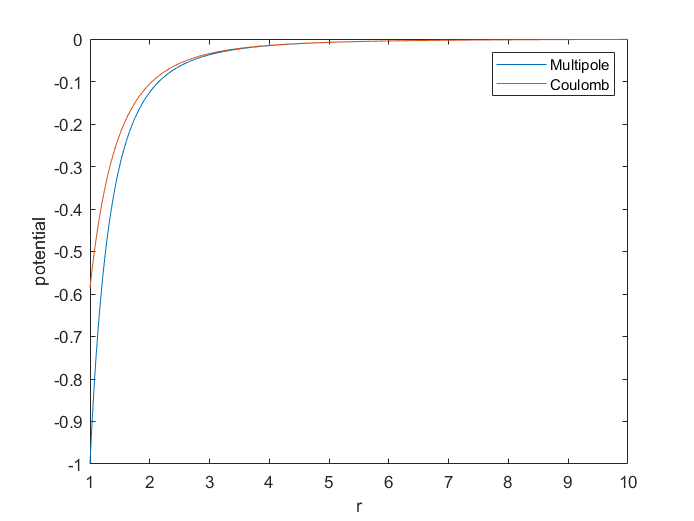
\includegraphics[width=0.8\textwidth]{4.png}\caption{The potential in the $z=0$ plane}
    \end{figure}
  \end{enumerate}

  \item \textbf{Dielectrics}: A point charge $q$ is located outside a dielectric sphere with dielectric constant $\epsilon$ as shown in the figure.
  \begin{enumerate}
    \item Calculate the electrostatic potential everywhere in space.
    \item Calculate the electric fields everywhere in space.
    \item Calculate the electric polarization in the dielectric sphere, and calculate the bound charge density at the surface induced by the polarization.
    \item Verify that, when $\epsilon$ is infinitely large, the system is equivalent to a conductor.
    \begin{figure}[h]
      \centering
      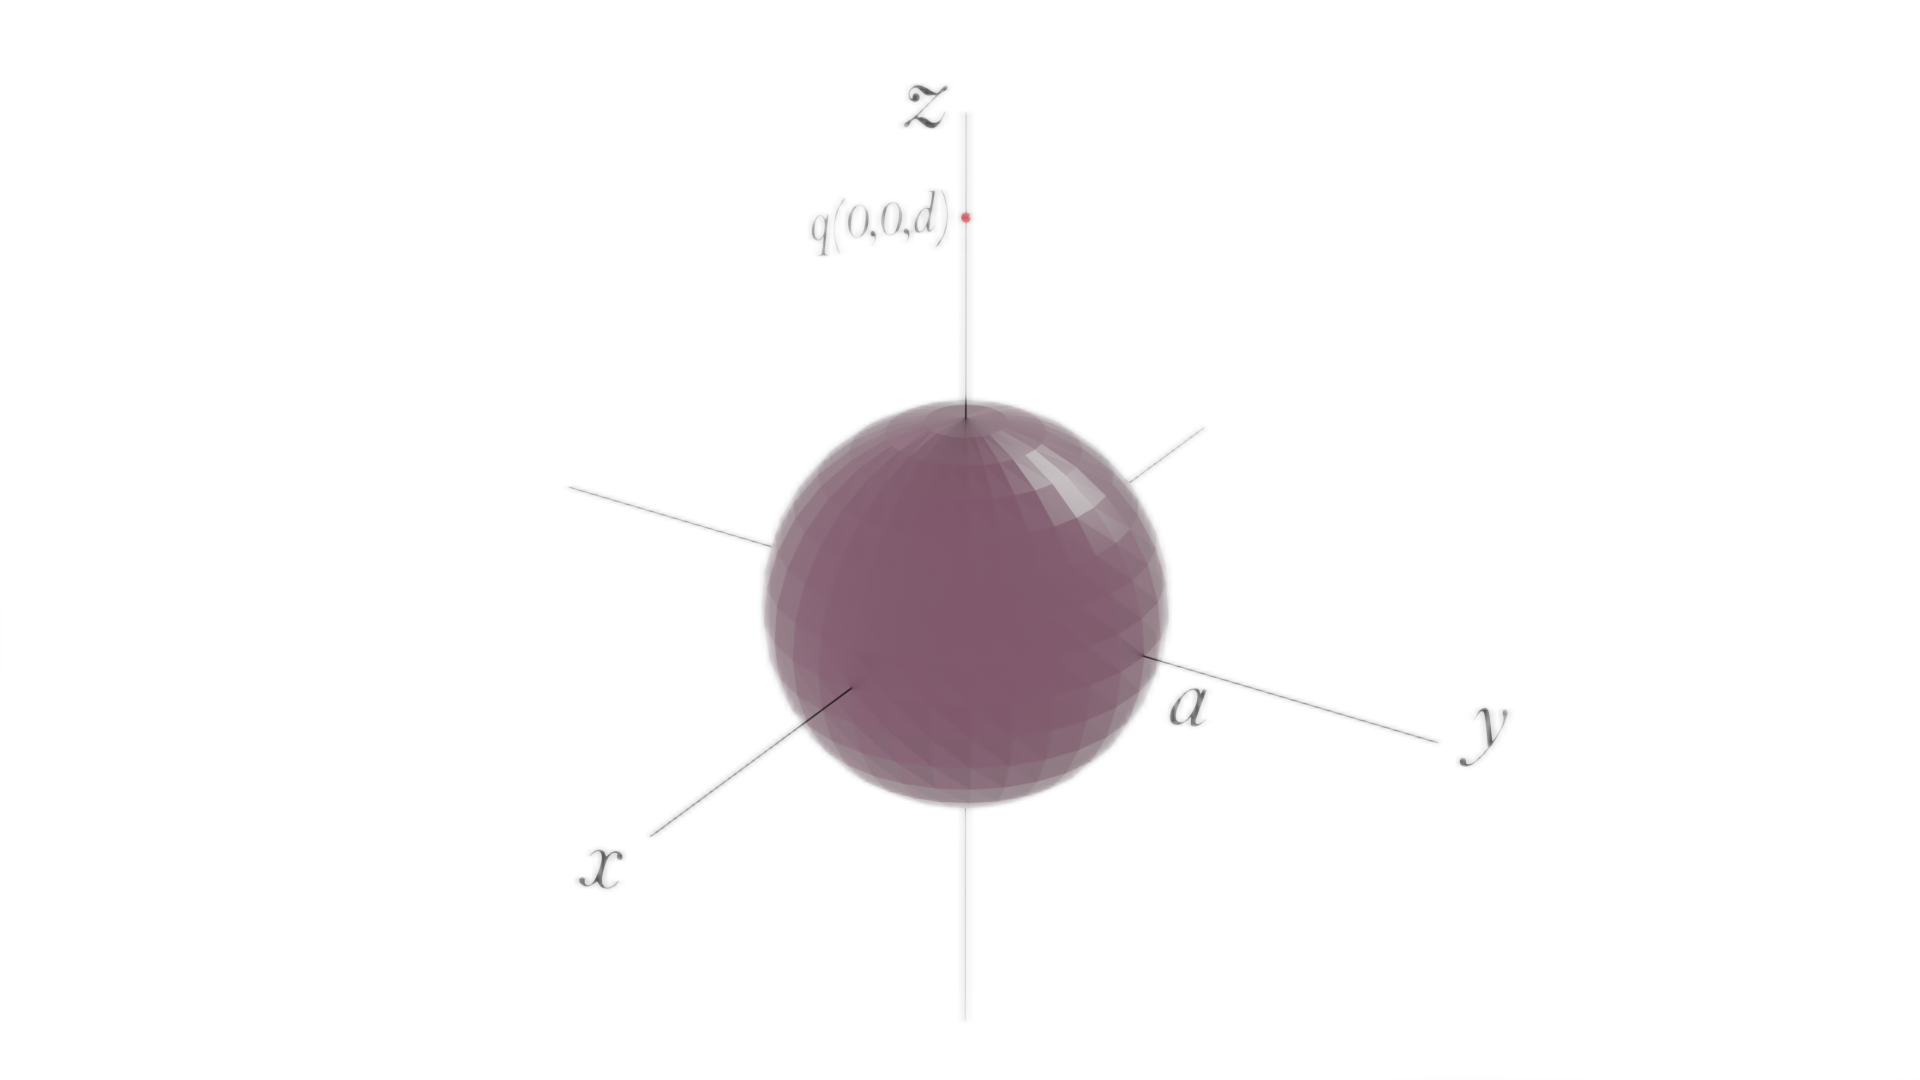
\includegraphics[width=0.6\textwidth]{3.png}
    \end{figure}
  \end{enumerate}
  \rule[0pt]{6cm}{0.05em}
  \begin{enumerate}
    \item From the expansion of the Green's function for a spherical shell bounded by $r=a$ and $r=b$
    \begin{eqnarray}
      G(\boldsymbol{r},\boldsymbol{r}')=4\pi\sum_{l=0}^{\infty}\sum_{m=-l}^{l}\dfrac{Y^*_{lm}(\theta',\phi')Y_{lm}(\theta,\phi)}{(2l+1)\left[1-(\dfrac{a}{b})^{2l+1}\right]}(r^l_{<}-\dfrac{a^{2l+1}}{r_{<}^{l+1}})(\dfrac{1}{r^{l+1}_{>}}-\dfrac{r^l_{>}}{b^{2l+1}})
    \end{eqnarray}
    
    Set $b\to\infty$, we obtain the Green's function appropriate for the ``exterior'' problem with a spherical boundary at $r=a$. Considering the symmetry, we hence obtain,
    \begin{eqnarray}
      \dfrac{1}{|\boldsymbol{r}-\boldsymbol{r}'|}=\sum_{l=0}^{\infty}\left[\dfrac{r^l_{<}}{r^{l+1}_{>}}-\dfrac{a^{2l+1}}{(r_{<}r_{>})^{l+1}}\right]
    \end{eqnarray}

    Since there's no point charge in the sphere, the potential satisfies the \textit{Poisson equation}. Thus we can set the general solution:
    \begin{eqnarray}
      \phi_1(\boldsymbol{r})&=&\begin{cases}
        \dfrac{q}{4\pi\epsilon_0}\sum\limits_{n}(\dfrac{r^n}{d^{n+1}}-\dfrac{a^{2n+1}}{r^{n+1} d^{n+1}})P_n(\cos\theta)+\sum\limits_{n}(a_n r^n+\dfrac{b_n}{r^{n+1}})P_n(\cos\theta)\quad\quad a<r<d\\
        \dfrac{q}{4\pi\epsilon_0}\sum\limits_{n}(\dfrac{d^n}{r^{n+1}}-\dfrac{a^{2n+1}}{r^{n+1} d^{n+1}})P_n(\cos\theta)+\sum\limits_{n}(a_n r^n+\dfrac{b_n}{r^{n+1}})P_n(\cos\theta)\quad\quad r>d
      \end{cases}\\
      \phi_2(\boldsymbol{r})&=&\sum\limits_{n}(c_n r^n+\dfrac{d_n}{r^{n+1}})P_n(\cos\theta)\quad\quad\quad\quad r\leqslant a
    \end{eqnarray}
    
    With the boundary condition:
    \begin{eqnarray}
      \left.\phi_1\right|_{r\to\infty}=const,&&\quad\quad \left.\phi_2\right|_{r=0}=const\\
      \left.\phi_1\right|_{r=a}=\left.\phi_2\right|_{r=a},&&\quad\quad \epsilon_0\left.\dfrac{\partial \phi_1}{\partial r}\right|_{r=a}=\epsilon\left.\dfrac{\partial \phi_2}{\partial r}\right|_{r=a}
    \end{eqnarray}

    Then,
    \begin{eqnarray}
      0&=&d_n=a_n\\
      \sum_{n}\dfrac{b_n}{a^{n+1}}P_n(\cos\theta)&=&\sum_{n}c_n a^n P_n(\cos\theta)\\
      \dfrac{q}{4\pi\epsilon_0}\sum_n(\dfrac{na^{n-1}}{d^{n+1}}+\dfrac{(n+1)a^{n-1}}{d^{n+1}})P_n(\cos\theta)-\sum_{n}\dfrac{(n+1)b_n}{a^{n+2}}P_n(\cos\theta)&=&\dfrac{\epsilon}{\epsilon_0}\sum_{n}nc_n a^{n-1}P_n(\cos\theta)\nonumber\\
    \end{eqnarray}

    The coefficients $c_n$ and $b_n$,
    \begin{eqnarray}
        c_n=\dfrac{q(2n+1)}{4\pi\left[\epsilon n+\epsilon_0(n+1)\right]d^{n+1}},\quad\quad b_n=\dfrac{q(2n+1)a^{2n+1}}{4\pi\left[\epsilon n+\epsilon_0(n+1)\right]d^{n+1}}
    \end{eqnarray}

    Hence, the potential is formed as 
    \begin{eqnarray}
      \phi_1(\boldsymbol{r})&=&\begin{cases}
        \dfrac{q}{4\pi\epsilon_0}\sum\limits_{n}(\dfrac{r^n}{d^{n+1}}-\dfrac{a^{2n+1}}{r^{n+1} d^{n+1}})P_n(\cos\theta)+\sum\limits_{n}\dfrac{q(2n+1)a^{2n+1}}{4\pi\left[\epsilon n+\epsilon_0(n+1)\right]d^{n+1}}\dfrac{1}{r^{n+1}}P_n(\cos\theta)\quad a<r<d\\
        \dfrac{q}{4\pi\epsilon_0}\sum\limits_{n}(\dfrac{d^n}{r^{n+1}}-\dfrac{a^{2n+1}}{r^{n+1} d^{n+1}})P_n(\cos\theta)+\sum\limits_{n}\dfrac{q(2n+1)a^{2n+1}}{4\pi\left[\epsilon n+\epsilon_0(n+1)\right]d^{n+1}}\dfrac{1}{r^{n+1}}P_n(\cos\theta)\quad r>d
      \end{cases}\nonumber\\
      ~\\
      \phi_2(\boldsymbol{r})&=&\sum\limits_{n}\dfrac{q(2n+1)}{4\pi\left[\epsilon n+\epsilon_0(n+1)\right]d^{n+1}}r^n P_n(\cos\theta)\quad\quad\quad\quad r\leqslant a
    \end{eqnarray}

    \item $\boldsymbol{E}(\boldsymbol{r})=-\nabla\phi$ gives
    \begin{eqnarray}
      \boldsymbol{E}_1(\boldsymbol{r})&=&
      \begin{cases}
        -\Big[\dfrac{q}{4\pi\epsilon_0}\sum\limits_{n}(\dfrac{n r^{n-1}}{d^{n+1}}+\dfrac{(n+1)a^{2n+1}}{r^{n+2}d^{n+1}})P_n(\cos\theta)-\sum\limits_{n}\dfrac{q(2n+1)a^{2n+1}}{4\pi\left[\epsilon n+\epsilon_0(n+1)\right]d^{n+1}}\dfrac{n+1}{r^{n+2}}P_n(\cos\theta)\Big]\hat{\boldsymbol{r}}\nonumber\\
        +\Bigl[\dfrac{q}{4\pi\epsilon_0}\sum\limits_{n}(\dfrac{r^n}{d^{n+1}}-\dfrac{a^{2n+1}}{r^{n+1} d^{n+1}})\dfrac{dP_n(\cos\theta)}{d\cos\theta}+\sum\limits_{n}\dfrac{q(2n+1)a^{2n+1}}{4\pi\left[\epsilon n+\epsilon_0(n+1)\right]d^{n+1}}\dfrac{1}{r^{n+1}}\dfrac{dP_n(\cos\theta)}{d\cos\theta}\Bigr](\dfrac{\sin\theta}{r})\hat{\boldsymbol{\theta}}\\
        ~\quad\quad\quad\quad\quad\quad\quad\quad\quad\quad\quad\quad\quad\quad\quad\quad\quad\quad\quad\quad\quad\quad\quad\quad\quad\quad\quad\quad\quad\quad\quad\quad\quad\quad\quad\quad a<r<d\\
        -\Big[\dfrac{q}{4\pi\epsilon_0}\sum\limits_{n}(-\dfrac{(n+1) d^{n}}{r^{n+2}}+\dfrac{(n+1)a^{2n+1}}{r^{n+2}d^{n+1}})P_n(\cos\theta)-\sum\limits_{n}\dfrac{q(2n+1)a^{2n+1}}{4\pi\left[\epsilon n+\epsilon_0(n+1)\right]d^{n+1}}\dfrac{n+1}{r^{n+2}}P_n(\cos\theta)\Big]\hat{\boldsymbol{r}}\nonumber\\
        +\Bigl[\dfrac{q}{4\pi\epsilon_0}\sum\limits_{n}(\dfrac{d^n}{r^{n+1}}-\dfrac{a^{2n+1}}{r^{n+1} d^{n+1}})\dfrac{dP_n(\cos\theta)}{d\cos\theta}+\sum\limits_{n}\dfrac{q(2n+1)a^{2n+1}}{4\pi\left[\epsilon n+\epsilon_0(n+1)\right]d^{n+1}}\dfrac{1}{r^{n+1}}\dfrac{dP_n(\cos\theta)}{d\cos\theta}\Bigr](\dfrac{\sin\theta}{r})\hat{\boldsymbol{\theta}}\\
        ~\quad\quad\quad\quad\quad\quad\quad\quad\quad\quad\quad\quad\quad\quad\quad\quad\quad\quad\quad\quad\quad\quad\quad\quad\quad\quad\quad\quad\quad\quad\quad\quad\quad\quad\quad\quad\quad r>d
      \end{cases}\nonumber\\
      \boldsymbol{E}_2(\boldsymbol{r})&=&
      -\Big[\sum\limits_{n}\dfrac{q(2n+1)n}{4\pi\left[\epsilon n+\epsilon_0(n+1)\right]d^{n+1}}r^{n-1} P_n(\cos\theta)\Big]\hat{\boldsymbol{r}}+\Bigl[\sum\limits_{n}\dfrac{q(2n+1)}{4\pi\left[\epsilon n+\epsilon_0(n+1)\right]d^{n+1}}r^n \dfrac{dP_n(\cos\theta)}{d\cos\theta}\Bigr]\dfrac{\sin\theta}{r}\hat{\boldsymbol{\theta}}\nonumber\\
      &&~\quad\quad\quad\quad\quad\quad\quad\quad\quad\quad\quad\quad\quad\quad\quad\quad\quad\quad\quad\quad\quad\quad\quad\quad\quad\quad\quad\quad\quad\quad\quad\quad\quad\quad\quad\quad\quad\quad r\leqslant a\nonumber\\
    \end{eqnarray}
    
    \item
    \begin{eqnarray}
      \boldsymbol{P}
      &=&(\epsilon-\epsilon_0)\boldsymbol{E}_2\nonumber\\
      &=&-\Big[\sum\limits_{n}\dfrac{(\epsilon-\epsilon_0)q(2n+1)n}{4\pi\left[\epsilon n+\epsilon_0(n+1)\right]d^{n+1}}r^{n-1} P_n(\cos\theta)\Big]\hat{\boldsymbol{r}}+\Bigl[\sum\limits_{n}\dfrac{(\epsilon-\epsilon_0)q(2n+1)}{4\pi\left[\epsilon n+\epsilon_0(n+1)\right]d^{n+1}}r^n \dfrac{dP_n(\cos\theta)}{d\cos\theta}\Bigr]\dfrac{\sin\theta}{r}\hat{\boldsymbol{\theta}}\nonumber\\
    \end{eqnarray}
    \begin{eqnarray}
      \sigma_{\boldsymbol{P}}
      &=&\left.\boldsymbol{P}\cdot\hat{\boldsymbol{r}}\right|_{r=a}\nonumber\\
      &=&-\Big[\sum\limits_{n}\dfrac{(\epsilon-\epsilon_0)q(2n+1)n}{4\pi\left[\epsilon n+\epsilon_0(n+1)\right]d^{n+1}}a^{n-1} P_n(\cos\theta)\Big]\nonumber\\
    \end{eqnarray}

    \item As $\epsilon\to\infty$
    \begin{eqnarray}
      \phi_2(\boldsymbol{r})\to 0,\quad\quad \boldsymbol{E}_2\to 0, \quad\quad\quad \phi_1(\boldsymbol{r})\to\begin{cases}
        \dfrac{q}{4\pi\epsilon_0}\sum\limits_{n}(\dfrac{r^n}{d^{n+1}}-\dfrac{a^{2n+1}}{r^{n+1} d^{n+1}})P_n(\cos\theta)\quad a<r<d\\
        \dfrac{q}{4\pi\epsilon_0}\sum\limits_{n}(\dfrac{d^n}{r^{n+1}}-\dfrac{a^{2n+1}}{r^{n+1} d^{n+1}})P_n(\cos\theta)\quad r>d
      \end{cases}
    \end{eqnarray}

    That is, the system degenerates as a conducted sphere which the potential is zero everywhere inside the sphere. Thus it becomes a perfect conductor, and the potential on the surface is bounded by zero. Hence the system is equivalent to a conductor.
  \end{enumerate}
\end{enumerate}


















\end{document}